\section{Experiments}\label{sec:exp}

\subsection{Design: three pre-registered studies}\label{sec:design}
% Sources: G5/EXPERIMENT_PROTOCOL.md (Study 1), S2/S2_PLAN.md (Study 2), S3/STUDY3_PLAN.md (Study 3), docs/tuning_spaces.md.
\paragraph{Settings and baselines.} The main claims concern LLP with random bags of 8 (ROC AUC) and PLL in which each
wrong class enters the candidate set independently with probability $q\in\{0.3,0.6\}$ (accuracy). Weak labels are
generated on the training part of stratified 70/30 splits (seeds 0--2) shared by all methods; datasets have 500 to
10{,}000 rows. Studies~1 and~2 run the peer-reviewed baselines of each setting, in their published defaults and tuned
by 20 random configurations scored on a validation split \emph{with weak labels only}: for LLP, DLLP \citep{dllp} with an
MLP or a linear model, LLP-VAT \citep{tsai2020llpvat}, EasyLLP \citep{easy_llp} and GLWS \citep{glws}; for PLL, PRODEN
\citep{proden}, GLWS/ILL \citep{glws,ill}, RC and CC \citep{feng2020provably}. With the same TFM
we also run the \emph{naive TFM} (one label per point consistent with the weak labels), \emph{hard-EM} (arg max instead
of sampling) and an \emph{oracle}. \ours{} is never tuned per dataset. A rule applied to development datasets fixed the
\emph{primary comparators}: linear DLLP and tuned CC.

\paragraph{Studies 1 and 2: one chain against specialised learners.} H2 (LLP) and H4 (PLL) require the single chain to
beat the primary comparator and the naive TFM (two-sided Wilcoxon signed-rank over datasets, Holm-adjusted) \emph{and}
to beat the baseline with the best mean score on $\ge$70\% of datasets (LLP), or to match or beat it on $\ge$60\% at each
level (PLL). H3 compares it with hard-EM on log loss (Bayesian signed-rank test \citep{benavoli2017bayesian}).
\emph{Study~1} used 24 OpenML-CC18 datasets \citep{bischl2021openml} with TabPFN~v2 as the registered TFM and TabICL~v2
as a registered ablation. \emph{Study~2} replicated it on \val{s2-n-total} new datasets from five curated suites
\citep[e.g.][]{grinsztajn2022tree} with TabICL~v2, changing nothing else (H2$'$--H4$'$).

\paragraph{Study 3: several starts and several TFMs.} \emph{Study~3} used \val{s3-n-total} further datasets
(\val{s3-n-binary} binary with LLP, \val{s3-n-multi} multiclass with PLL at $q=0.6$) from the same suites, OpenML-CC18
and TabArena \citep{tabarena}, excluding every dataset used earlier and TabDPT's pretraining sets. It ran TabICL~v2,
TabPFN-3 \citep{tabpfn3} and TabDPT \citep{tabdpt} on all datasets and TabPFN~v2 on the \val{s3-n-pfn2} within its
published limits. Per dataset, $\delta_1$ is the mean over TFMs of (multi-start $-$ single chain), and $\delta_2$ is the
multi-TFM score minus the mean over TFMs of the multi-start score, the expected score of a TFM picked at random.
H1$''$: $\delta_1>0$; H2$''$: $\delta_2>0$ (one-sided Wilcoxon signed-rank, Holm-adjusted). Three criteria were
registered without a test. H3$''$: a diagnostic computed without labels identifies the cells in which the single chain
fails (AUC $\ge0.80$). C4$''$: the multi-start sampler is more than 0.02 below the better of the single chain and the
tuned learner $L$ in at most 10\% of (TFM, dataset) pairs. C5$''$: the multi-TFM average is on average within 0.01 of
the best TFM of each dataset and more than 0.02 behind it on at most 3. The only baseline of Study~3 is $L$ (tuned
DLLP-MLP and tuned CC, the strongest LLP baseline and the primary PLL comparator of Study~2). All protocols were
committed before the evaluation tables were downloaded, and development between the studies was exploratory
(\cref{app:prereg,app:dev}).

\begin{table}[t]
\centering
\caption{Studies 1 and 2, pre-registered tests of the single chain. $\Delta$: mean over datasets of (\ours{} $-$
comparator), 3 seeds each; W/T/L: datasets won/tied/lost; $p_{\mathrm{Holm}}$: two-sided Wilcoxon signed-rank,
Holm-adjusted within each hypothesis. Bold: significant in favour of \ours{}.}
\label{tab:main}
\setlength{\tabcolsep}{3.2pt}
\resizebox{\textwidth}{!}{% generated by paper/scripts/make_tables.py — do not edit
\begin{tabular}{@{}lllrrrrrr@{}}
\toprule
 & & & \multicolumn{3}{c}{Study 1: TabPFN v2} & \multicolumn{3}{c}{Study 2: TabICL v2, new datasets} \\
\cmidrule(lr){4-6}\cmidrule(l){7-9}
Setting & Metric & Gibbs vs. & $\Delta$ & W/T/L & $p_{\mathrm{Holm}}$ & $\Delta$ [95\% CI] & W/T/L & $p_{\mathrm{Holm}}$ \\
\midrule
LLP, bag size 8 & AUC & DLLP (linear) & +0.024 & 8/0/2 & 0.232 & +0.052 [+0.024, +0.086] & 16/0/2 & \textbf{\ensuremath{<}0.001} \\
 &  & Naive TFM & +0.148 & 10/0/0 & \textbf{0.004} & +0.116 [+0.085, +0.150] & 18/0/0 & \textbf{\ensuremath{<}0.001} \\
\addlinespace
PLL, $q=0.3$ & Acc. & CC (tuned) & +0.022 & 10/0/4 & 0.084 & +0.012 [+0.006, +0.019] & 8/2/0 & \textbf{0.016} \\
 &  & Naive TFM & +0.099 & 13/0/1 & \textbf{\ensuremath{<}0.001} & +0.022 [+0.012, +0.033] & 10/0/0 & \textbf{0.008} \\
\addlinespace
PLL, $q=0.6$ & Acc. & CC (tuned) & \ensuremath{-}0.132 & 7/0/7 & 0.715 & +0.012 [+0.006, +0.019] & 8/1/1 & \textbf{0.016} \\
 &  & Naive TFM & +0.180 & 12/0/2 & \textbf{0.002} & +0.205 [+0.094, +0.337] & 10/0/0 & \textbf{0.008} \\
\midrule
\multicolumn{3}{@{}l}{Pre-registered verdict} & \multicolumn{3}{l}{H2: not met; H4: not met} & \multicolumn{3}{l}{H2$'$: met; H4$'$: met} \\
\bottomrule
\end{tabular}
}
\end{table}

\subsection{One chain with a robust TFM outperforms specialised learners}\label{sec:s2}
In Study~2 all pre-registered tests passed (\cref{tab:main}, right; \cref{app:s2-s1}). On LLP the single chain improved
AUC over linear DLLP by \val{s2-llp-cmp-diff} \val{s2-llp-cmp-ci} (\val{s2-llp-cmp-wtl}) and beat the strongest LLP
baseline, \val{s2-llp-strongest-name}, on \val{s2-llp-strongest-wins} datasets \claim{6}. On PLL it improved accuracy
over tuned CC by \val{s2-pll3-cmp-diff} at $q=0.3$ and \val{s2-pll6-cmp-diff} at $q=0.6$, was at least as accurate as
the strongest PLL baseline on \val{s2-pll3-rule60} and \val{s2-pll6-rule60} datasets, and stayed within
\val{s2-pll3-oracle-gap} and \val{s2-pll6-oracle-gap} accuracy points of the oracle \claim{8}. With the same TFM and
warm start it had lower log loss than hard-EM in \val{s2-h3-frac} of \val{s2-h3-cells} cells (Study~1:
\val{s1-h3-frac} of \val{s1-h3-cells}) \claim{7}: the gain comes from sampling the labels jointly. The gain over the
naive TFM is large for candidate sets and bag counts and absent where naive labels carry all the information
(\cref{app:secondary}) \claim{12}.

\subsection{Stalling, and what the response map explains}\label{sec:tfm}
Study~1, with TabPFN~v2, did not meet its criteria (\cref{tab:main}, left). \ours{} improved on the naive TFM by
\val{s1-llp-naive-diff} AUC on LLP and \val{s1-pll3-naive-diff} and \val{s1-pll6-naive-diff} accuracy on PLL, and led
the primary comparators on LLP and on PLL at $q=0.3$, short of significance. At $q=0.6$ it was ahead on ten datasets by
\val{s1-pll6-rest-diff} on average, while on the four with at least eight classes the chains stalled near an
uninformative labelling (\cref{fig:mechanism-full}), which turned the average into a deficit of
\val{s1-pll6-cmp-diff}.

\Cref{fig:mechanism} shows the gain $\Phi(r)-r$ of one sweep started from an assignment with a fraction $r$ of
correct labels and uniformly placed errors. With TabPFN~v2 it is negative for intermediate $r$ on all four datasets:
by \cref{thm:basins}(b), a chain that starts there cannot climb. With TabICL~v2 it is positive throughout; in the
registered ablation on the same datasets the sampler with TabICL~v2 did not stall and passed every test
(\cref{app:s1-tabicl}), and Study~2 then tested that TFM prospectively \claim{13}.

\paragraph{Does the assumption hold?} We checked \cref{ass:H} on \val{v2-p8-n} cells of development runs (TabPFN~v2 and
TabICL~v2; exploratory, thresholds written before the runs, \cref{app:dev}). The fixed point of the uniform-error map
predicts the final label accuracy of a chain with a median error of \val{v2-p9-uniform}: right about direction, not
about level. With TabPFN~v2 the error is one-sided: chains do better than the map says, so only the lower half of the
assumption holds, and the uniform map certifies that a chain will climb, not that it will stall. With errors placed according to the chain's own marginals instead, the fixed point predicts the final accuracy with a median error of \val{v2-p8-med}
(\cref{fig:chainmap}) \claim{17}. This checks the one-dimensional description; it is not a forecast, because the
marginals come from the chain whose end is predicted and both maps need true labels. Under uniform errors TabPFN-3 has
a negative gain at low accuracy on \val{v2-p11-pfn3-low} of the four datasets and TabDPT on \val{v2-p11-tabdpt-low}.

\begin{figure}[t]
\centering
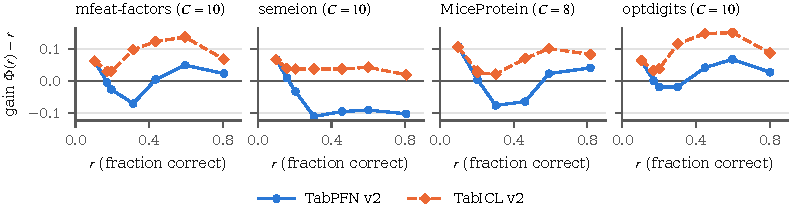
\includegraphics[width=\textwidth]{figures/mechanism_map}
\caption{Response maps for PLL at $q=0.6$ on the four Study~1 datasets with at least eight classes: gain $\Phi(r)-r$ of
one Gibbs sweep started from a fraction $r$ of correct labels, errors placed uniformly (3 seeds; needs true labels).}
\label{fig:mechanism}
\end{figure}

\subsection{Several starts and several TFMs}\label{sec:s3}
\begin{table}[t]
\centering
\caption{Study 3 (\val{s3-n-total} new datasets, four TFMs, 3 seeds). Left: registered hypotheses and criteria
(\cref{sec:design}); mean over datasets [bootstrap 95\% interval], W/T/L, one-sided Wilcoxon signed-rank $p$,
Holm-adjusted. Right: mean test score of the single chain and the multi-start average. $^\dagger$TabPFN~v2 ran only on
\val{s3-pfn2-nllp} LLP and \val{s3-pfn2-npll} PLL datasets; its row is not comparable with the others.}
\label{tab:s3}
\setlength{\tabcolsep}{3pt}
\resizebox{\textwidth}{!}{\begin{tabular}{@{}c@{\hspace{1.2em}}c@{}}% generated by paper/scripts/make_v2.py — do not edit
\begin{tabular}{@{}llll@{}}
\toprule
 & Statement & Result & Outcome \\
\midrule
H1$''$ & multi-start $>$ single chain & +0.058 [+0.016, +0.114], 13/6/1, $p$\ensuremath{<}0.001 & \textbf{confirmed} \\
H2$''$ & multi-TFM $>$ a TFM drawn at random & +0.046 [+0.019, +0.079], 18/2/0, $p$\ensuremath{<}0.001 & \textbf{confirmed} \\
H3$''$ & diagnostic AUC $\ge 0.80$ & 0.766 [0.59, 0.92] & not confirmed \\
C4$''$ & regressions $\le 10\%$ & 10/71 (14.1\%) & not met \\
C5$''$ & multi-TFM $\approx$ best TFM & gap 0.000; 1/20 worse by $>0.02$ & met \\
\bottomrule
\end{tabular}
 & % generated by paper/scripts/make_v2.py — do not edit
\begin{tabular}{@{}lrrrr@{}}
\toprule
 & \multicolumn{2}{c}{LLP, AUC (12)} & \multicolumn{2}{c}{PLL, acc.\ (8)} \\
\cmidrule(lr){2-3}\cmidrule(l){4-5}
TFM & single & multi & single & multi \\
\midrule
TabICL~v2 & 0.802 & 0.803 & 0.749 & 0.805 \\
TabPFN-3 & 0.817 & 0.817 & 0.371 & 0.650 \\
TabDPT & 0.786 & 0.799 & 0.648 & 0.720 \\
TabPFN~v2$^\dagger$ & 0.784 & 0.798 & 0.488 & 0.494 \\
\midrule
Multi-TFM & & \textbf{0.828} & & \textbf{0.808} \\
Tuned learner $L$ & \multicolumn{2}{c}{0.783} & \multicolumn{2}{c}{0.717} \\
\bottomrule
\end{tabular}
\end{tabular}}
\end{table}

\paragraph{Confirmed.} Both hypotheses of Study~3 passed (\cref{tab:s3}; per dataset in \cref{fig:s3}). Averaging three starts
improved on the single chain by \val{s3-h1-mean} on average (\val{s3-h1-wtl} datasets) \claim{14}. The gain is
concentrated: \val{s3-h1-pll} on PLL against \val{s3-h1-llp} on LLP, a median of \val{s3-h1-median} over all datasets,
and largest where single chains stall (TabPFN-3 on PLL: \val{s3-v1-tabpfn_v3-pll} to \val{s3-A1-tabpfn_v3-pll}). The
multi-TFM average improved on a TFM picked at random by \val{s3-h2-mean} (\val{s3-h2-wtl}) and was level with the best
TFM of each dataset (mean gap \val{s3-c5-gap}), more than 0.02 behind it once (\val{s3-c5-worst-name}:
\val{s3-c5-worst-X} against \val{s3-c5-worst-best}) \claim{15}. Both tests also pass without the five flagged datasets
($p_{\mathrm{Holm}}=\val{s3-s1-h1-p}$ and \val{s3-s1-h2-p}).

\paragraph{Not confirmed.} The diagnostic of H3$''$, the mean total-variation distance between the label marginals of
the warm-start and learner-start chains, reached an AUC of \val{s3-h3-auc}, below the registered 0.80. It separated
failures for TabPFN-3 (\val{s3-h3-auc-tabpfn_v3}) and TabICL~v2 (\val{s3-h3-auc-tabicl_v2}) but not for TabDPT
(\val{s3-h3-auc-tabdpt}) or TabPFN~v2 (\val{s3-h3-auc-tabpfn_v2}): we have no label-free diagnostic that transfers
across TFMs. C4$''$ also failed: with one TFM, the multi-start sampler was more than 0.02 behind the better of its
single chain and $L$ in \val{s3-c4-n} of \val{s3-n-pairs} pairs, in \val{s3-c4-vs-v1} of them behind the single chain
and in \val{s3-c4-vs-L} behind $L$ (\cref{app:s3}) \claim{18}. One TFM with several starts is thus not guaranteed to
match a tuned specialised learner; their registered descriptive comparison was not significant (\val{s3-a1L-mean},
$p=\val{s3-a1L-p}$).

\paragraph{Exploratory analysis.} The following was not registered and was computed after the confirmatory scoring
(\cref{app:s3}). (i) The multi-TFM average was above $L$ on all \val{s3x-X-L-w} datasets, by \val{s3x-X-L-mean} on
average \val{s3x-X-L-ci}, and by the measure of C4$''$ it regressed in \val{s3x-X-reg} of \val{s3-n-pairs} pairs; even
the average of single chains over TFMs, with no trained model, was above $L$ on \val{s3x-Xwarm-L-w} datasets \claim{19}.
(ii) The benefit of several starts comes from the learner start: the chain started from $L$ alone matches the
three-start average (\val{s3x-base-A1}), the cold start adds little, and averaging the single chain with $L$'s own
prediction, with no further chain, does as well as the registered average (\val{s3x-warmL-A1},
$p=\val{s3x-warmL-A1-p}$). (iii) The three chains ended within 0.03 of each other in label accuracy in
\val{s3x-basin-same} of cells; the PLL gain of the multi-start average is \val{s3x-basin-G-pll-diff} in the other cells
and \val{s3x-basin-G-pll-same} where chains agree, as \cref{thm:basins} suggests. (iv) TabICL~v2 carries much of the
multi-TFM result: the average is not significantly better than TabICL~v2's own multi-start average
(\val{s3x-X-A1-tabicl_v2}, $p=\val{s3x-X-A1-tabicl_v2-p}$); averaging over TFMs buys not having to know this in advance.

\subsection{Real weak labels, exactness and cost}\label{sec:real}\label{sec:ablation}
On three real partial-label datasets (BirdSong, Lost, MSRCv2; 10 random 90/10 splits; single chain with TabICL~v2,
registered in Study~1), \ours{} had the highest mean accuracy on all three and the best mean rank among
\val{s1-real-nmethods} methods (\val{s1-real-rank-pooled}; \cref{tab:real}) \claim{9}. The MH-corrected block sampler,
exact when the TFM is, did not predict better than the default at the same 30 sweeps (with TabICL~v2:
\val{s2e-mh-llp} AUC on LLP, \val{s2e-mh-pll6} accuracy on PLL at $q=0.6$; \cref{tab:s2e}) and was a median
\val{s2e-mh-cost-median} times slower; the comparison confounds bias with slower mixing. Chains do not mix at the level
of individual labels, and in an exploratory rerun of Study~2 with a second chain H4$'$ at $q=0.6$ no longer passes
($p_{\mathrm{Holm}}=\val{r4-b-pll6-p}$), while with the two chains averaged every test passes (\cref{tab:r4}): that
result depends on Monte Carlo variation, which averaging reduces.
On one T4 GPU a chain took a median of \val{s2-cost-median-s}\,s in Study~2 and between
\val{s3x-cost-sec-tabicl_v2}\,s (TabICL~v2) and \val{s3x-cost-sec-tabpfn_v2}\,s (TabPFN~v2) in Study~3; all chains of the
four-TFM average took a median of \val{s3x-cost-X-min} minutes per dataset and seed \claim{11}.
